\section{Pascal Analyzer} \label{sec:pascal_analyzer}
High-performance computing systems have become increasingly dynamic, complex, and unpredictable. To help build software that uses full-system capabilities, performance measurement and analysis tools exploit extensive execution analysis focusing on single-run results. Despite being effective in identifying performance hotspots and bottlenecks, these tools are not sufficiently suitable to evaluate the overall scalability trends of parallel applications. Either they lack the support for combining data from multiple runs or collect excessive data, causing unnecessary overhead. 
In this work, we present a tool for automatically measuring and comparing several executions of a parallel application according to various scenarios characterized by the input arrangements, the number of threads, number of cores, and frequencies.
%In this work, we present a tool for measuring and comparing several executions of a parallel application automatically with different input arrangements, number of threads, cores, and frequencies to understand its scalability by observing how it uses the available computational resources across configurations. 
Unlike other existing performance analysis tools, the proposed work covers some gaps in specialized features necessary to better understand computational resources scalability trends across configurations. 
%The proposed work covers some gaps and unspecialized features of existing performance analysis tools. 
%The tool features automatic instrumentation and direct mapping of parallel regions, accuracy-preserving data reductions, and ease of use to compare multiple configurations for improving analysis and productivity. 
In order to improve scalability analysis and productivity over the vast spectrum of possible configurations, the proposed tool features automatic instrumentation, direct mapping of parallel regions, accuracy-preserving data reductions, and ease of use.
%In addition, it aims at parallel scalability, instead focus on single-run performance, aggregating a minimal level of intrusion (<1\% on average), which is fundamental for accurately understanding the behavior and scalability trends of the parallel application.
As it aims at accurately understanding scalability trends of parallel applications, detailed single-run performance analyses show minimal intrusion (less than 1\% overhead).

\section{Introduction to profiling tools} \label{sec:introduction_to_profiling_tools}

Developing parallel programs capable of exploiting the computational power of high-performance systems is as well-known as it is challenging~\cite{Huck2007, Islam2019, Weber2019}. 
During the development process, the code optimization step is a fundamental part of the software construction strategy and is supported by performance measurement and analysis tools~\cite{Bergel2019, Weber2019, Huck2005, Geimer2010, Shende2006, Adhianto2010, Miller1995, Galobardes2015, Pillet2007, Islam2019}. The main objective of these tools is to help developers understand the execution characteristics, allowing the identification of bottlenecks and behavioral phenomena that compromise the program’s efficiency, thus guiding possible improvements~\cite{Brink2020, Huck2007}.

Nowadays, due to the complexity of parallel systems, correctly identifying and locating performance and scalability bottlenecks depends on the developer's ability to compare several measurements in different execution configurations~\cite{Bergel2019, Silva2018}. This investigative process tends to be tedious and complex, requiring in-depth knowledge of the problem domain, parallel systems, and measurement and analysis tools. 
%Mastering the analysis tools becomes necessary mainly because they differ from each other in terms of measurement strategy, the collected metrics, and the many points and focus of observation. 
Mastering the analysis tools is necessary because they differ from each other in terms of measurement strategy, metrics collected, and the many points and focus of observation.
Even though some solutions propose organizing and combining metrics from different sources, these distinct characteristics can compel developers to exploit more than one tool depending on their analysis~interests.

%Despite their differences, every existing tool has its own contributions in helping to understand the inner working of a program, and some can present a vast and varied set of metrics with a high degree of detail. 
Every existing tool has its own contributions in helping to understand the inner working of a program. Some can present a vast and varied set of metrics with a high degree of detail. 
However, developers may have difficulty using these tools when their interest is in analyzing parallel scalability. 
%The main challenge arises from the focus on investigating a single run, because scalability analysis requires contrasting runs of different configurations. 
The main challenge arises from the emphasis on studying a single run because scalability analysis requires contrasting runs of different configurations.
%In this sense, it tends to be more significant to measure and compare only a few data across executions of multiple configurations than to collect a vast amount of finer-grain data of single-configuration runs.
In terms of productivity, measuring and comparing only a few data between runs of multiple configurations tends to be more significant to scalability analysis than collecting a vast amount of finer-grain data of single-configuration runs.
Furthermore, due to the number of measurements, there is a natural overhead associated with the execution of the analysis tool itself. Some works indicate this overhead can reach 40\% of the program runtime, which influences and damages the observation of its efficiency variation~\cite{Eriksson2016}.
As such, a measurement and analysis approach that uses only the data needed to understand the application's efficiency variation can be advantageous. First, because measuring and collecting only the necessary data limits the degree of intrusion and, second, because this strategy makes the analysis tool simpler and easier to use. 
%Finally, the tool's availability can also be a drawback as some apply to specific compilers and execution frameworks. Indeed, the framework version is a limitation for some traditional tools like HPCToolkit~\cite{Adhianto2010} and TAU (Tuning and Analysis Utilities)
%MDPI: Is this an abbreviation? If affirmative, please add the explanation. Please carefully check and confirm -- INCLUDED ON THE NEXT PARAGRAPH
~\cite{Shende2006}.


From this context, we present a measurement tool that focuses on analyzing the parallel scalability of programs. It primarily provides runtime and power consumption measures in an approach that favors inspection of the overall behavior of the program before starting a more in-depth investigation of points that naturally require more detail, time and effort.
The work explores and combines strategies already used in other solutions, such as tracing, post-mortem analysis, and automatic instrumentation based on shared libraries. Additionally, it includes an instrumentation model that automatically relates parallel code regions to analysis regions, using a measurement strategy based on the intrinsic and primary behavior of the parallel frameworks. Due to this approach, the tool allows analyzing programs developed for shared-memory environments regardless of the compiler or framework versions. 
The framework version, which in some cases also requires specific compiler versions, is a limitation for some traditional tools like HPCToolkit~\cite{Adhianto2010} and TAU (Tuning and Analysis Utilities)~\cite{Shende2006}.

The proposed tool uses a tracing-based measurement technique to identify and measure the boundaries of the analysis regions. The tracing approach supports a hierarchical region analysis model allowing users to see how the efficiency of inner parts can impact the program's overall scalability. In addition, the tool uses an aggregation feature to reduce the volume of data produced while preserving accurate analysis capability with minimal overhead. The tool also includes usability features that reduce the developer's efforts during the measurement and analysis process. These features allow one to automate the process of running and merging data collected from multiple configurations, bypassing manual efforts and avoiding the drawbacks of non-computer-oriented analysis. 
%The tool does not display visuals elements natively. Still, its interface allows the collected data to be exported and viewed from the control terminal in tabular form. Data exported via the interface are organized into data frames that can be interpreted by other tools or even rendered directly from graphic libraries.
The collected data, available from the terminal in tabular form, can be exported as data blocks that can be interpreted by other tools or even rendered by graphics libraries to facilitate the visualization and data analysis.


%The proposed tool is an alternative for realizing parallel scalability analysis more efficiently than single-run-centric performance measurement and analysis tools. 
We offer an alternative tool for realizing parallel scalability analysis more efficiently than single-run-centric performance measurement and analysis tools. In addition to that, our framework can also be used to promote energy-aware software; methods that rely on accurate and efficient energy collection could benefit from energy consumption data for the entire program and specific regions of the application \cite{10.1007/978-3-319-58667-0_22,10.1007/978-3-319-58667-0_21,7016382,10.1145/3321551}. To summarize, the main contributions of this work are:

\begin{itemize}
	\item A lightweight automated process of measuring and comparing runs with different configurations.
	\item Transparent linking of parallel code sections to analysis regions.
	\item Hierarchical views and degrees of efficiency for the inner parts of a program.
	\item The imposed overhead is low and minimally intrusive, mainly because of the measurement approach and the number of metrics collected.
	\item It provides energy consumption measures for the different configuration parameters. 
\end{itemize}

The following sections describe how the tool is built and used for performance analysis. Section \ref{sec:state_of_the_art_profiling_and_tracing_tools} presents the related works. Section \ref{sec:pascal_architecture} describes the tool architecture and goals; it explains the main features, usage, and collected data. The experimental results are presented in Section \ref{sec:pascal_framework_validation}. Finally, the contributions are summarized in Section \ref{sec:conclusions_pascal}, with an outlook of future works.

\section{State of the art: profiling and tracing tools} \label{sec:state_of_the_art_profiling_and_tracing_tools}

Performance analysis aimed at code optimization is an essential activity for developing parallel applications with scalable performance. For this purpose, performance analysis tools, like Caliper~\cite{Boehme2016}, HPCToolkit~\cite{Adhianto2010}, Scalasca~\cite{Geimer2010}, TAU~\cite{Shende2006}, Vampir~\cite{Weber2019}, and VTune~\cite{Intel2021Vtune}, are useful because they help developers identify where the application uses the available computing resources inefficiently through collecting detailed data of its execution. Such tools differ from each other mainly in terms of data measurement and analysis strategy: tracing or profiling, post-mortem or real-time; individual or comprehensive observation focus; and for providing or not providing visual elements that facilitate the judgment of collected data. Other solutions, like the DASHING framework~\cite{Islam2019} and the HATCHET library~\cite{Brink2020}, allow inspection of performance data from multiple sources. In this case, the goal of DASHING and HATCHET is to provide a more robust data set to support the analysis process.

In the performance analysis process, observing the parallel program's execution as a sequence of events representing significant activities is essential to understand its behavior~\cite{Pantazopoulos1997}. Events are basic units of the analysis process, and the way they are observed influences strategies for collecting performance data. Profiling-based analysis tools collect information from events that occurs in the program execution and commonly operate by statistical sampling using interruptions. These interruptions can be caused, for example, by periodic breaks or hardware events. Interruptions allow checking the system state and the information collected depends on the focus of observation. Profiling-based tools use statistical techniques to describe the program behavior in terms of aggregate performance metrics. They usually ignore the chronology of events, but are known to be useful for identifying, for example, load imbalance, high communication time, or excessive routine calls. Paradyn~\cite{Miller1995}, and Periscope~\cite{Gerndt2010} are tools that adopt this strategy.

On the other hand, tracing-based analysis tools collect performance data from events that occur when the program takes over a particular state. Tracing can provide valuable information about the time dimension of a program, allowing users to check when and where transitions of routines, communications, and specific events occur. This measurement strategy tends to be more invasive and intrusive, generating a larger dataset than the profiling-based approach. Vampir~\cite{Weber2019} and Paraver~\cite{Labarta2005} are examples of this group. Some tools like HPCToolkit~\cite{Adhianto2010}, Scalasca~\cite{Geimer2010}, TAU~\cite{Shende2006} and VTune~\cite{Intel2021Vtune} support both profiling and~tracing.

%In this work we propose tracing to measure the program and identify when parts of its code were executed. 
In this work we propose tracing to identify when parts of a code were executed. 
%To mitigate some of the disadvantages usually related to tracing, the tool implements features such as automatic instrumentation mode and aggregation resource, in addition to adopting an analysis based only on time. 
To mitigate some of the disadvantages related to tracing, in addition to adopting a time-based analysis, the tool implements features such as automatic instrumentation mode and resources aggregation.
%The automatic instrumentation mode makes it possible for users to analyze the program's execution without modifying the compiled code. 
Our automatic instrumentation mode allows users to analyze program execution without modifying the source or the executable.
Although many other analysis tools use the automatic instrumentation mode, this work presents a different way of mapping and measuring the code parts. 
%In our proposal, parallel regions are the main focus of analysis, and there is no limitation on the version of OpenMP used in the development, as in tools such as HPCToolkit~\cite{Adhianto2010} and TAU~\cite{Shende2006}. 
In our proposal, parallel regions are the main focus of analysis. 
%The strategy is efficient in identifying the scalability trend of parts or the whole parallel program in execution.
The strategy is effective enough to identify the scaling trends of parts or of the entire running parallel program.
%Furthermore, collecting only data related to runtime reduces the associated overhead with the measurement process. 
Furthermore, collecting only specific runtime data reduces the overhead associated with the measurement process.
As with other similar tools, such as HPCToolkit~\cite{Adhianto2010} and TAU~\cite{Shende2006}, there is no limitation on the version of OpenMP~used.

Runtime overhead is an attribute associated with the set of additional instructions that are executed to collect the program measurements. The time to perform this ``extra code'' varies in line with the tool and is directly related, in quantity and degree of detail, to the aspects it measures. 
Limiting this overhead is crucial because it can compromise the understanding of program behavior, and divert optimization efforts to less effective points. 
According to some comparative and practical studies in this regard, tests on traditional tools have shown a runtime overhead ranging from 2\% to 40\%~\cite{Eriksson2016}.
%Fundamental to the proposal of this work, the overhead presented by the proposed tool differs according to the program under analysis but can be considered negligible (<1\%) for analyzing scalability trends of parallel applications.
Although different depending on the program analyzed, the overhead resulting from our instrumentation strategy can be considered negligible (less than 1\%) and optimal for analyzing trends in parallel applications.

Several performance analysis tools employ a post-mortem approach. 
%In this kind of approach, the tools collect performance metrics during the program execution, but the data interpretation is carried out only after its execution. 
In this case, the tool performs performance measurements and data collection while the program is running, and then the collected data will be interpreted.
HPCToolkit~\cite{Adhianto2010}, Scalasca~\cite{Geimer2010}, TAU~\cite{Shende2006} and VTune~\cite{Intel2021Vtune} are examples of post-mortem performance analysis tools. 
%Post-mortem performance analysis tools may require the storage of large volumes of performance data, but they are more suitable to provide an overall view of the execution. 
Depending on the type of analysis, these tools may require storing large amounts of data, but they are best suited to provide an overall view of the execution.
%On the other hand, real-time analysis tools enable performance analysis during the execution of the program. 
In contrast, run-time analysis tools perform both operations at run time.
This approach allows detecting waiting states and communication inefficiencies accurately. 
%However, an online analysis environment usually requires the coordinated usage of extra tools, which increases the analysis infrastructure complexity. 
Periscope~\cite{Gerndt2010} and Paradyn~\cite{Miller1995} are examples of tools in this group.
However, run-time analysis generally requires the coordinated action of tools, which increases the structural complexity.
%The need for synchronous initialization, communication between all resources used in the analysis, and the additional load on the network are disadvantages of the real-time approach. 
The need for synchronous initialization and communication between analysis resources as well as their impact on the runtime environment are the drawbacks of this approach.
%In addition, the analysis that depends on data collected at the end of the program's execution, as in the case of scalability analysis, are potentially damaged by the infrastructure overhead and do not, in practice, benefit from characteristics of real-time tools. 
In addition, the analysis, particularly that of scalability, which relies on the data collected at the end of the execution, is potentially degraded by the infrastructure overhead and therefore does not benefit from the characteristics of real-time tools.


\textls[-15]{Energy management solutions can also provide similar features for example GEOPM~\cite{10.1007/978-3-319-58667-0_21},} allows the measurement of time and energy of specific regions. The main advantage that we could not find in any other framework is that our tool can provide specific data of energy consumption of parallel regions in a completely automated way. For example, in GEOPM, it is necessary to instrument the source code to obtain the same result.

%To investigate the scalability trend, it is more important to identify the program's general behavior than its state at a given moment of execution. 
%Although the current performance analysis tools are helpful and allow to identify numerous aspects regarding the program's behavior, none of them presents characteristics directly focused on observing the scalability trend of parallel code. An indispensable feature for this purpose includes automating the program's measurement process in different configurations because a more accurate understanding of scalability requires measuring and comparing multiple code runs.
%Focused on more practical and objective analysis, we propose an alternative tool to observing a parallel program's scalability trend. It collects only information that allows deriving the overall program runtime, or parts of it, according to the user's interest, and includes relevant functionalities to an efficient measurement and analysis process. Among the supported features it provides: the automation of program runs based on different parameters; the generation of data sets that contain metrics with different execution parameters; and the reduction of the generated data volume on disk.

%Although the current performance analysis tools are helpful and allow to identify numerous aspects regarding the program status, to investigate scalability trends, it is more important to identify the behavior of parallel code rather than its state at a given moment of the execution, therefore the post-mortem approach is more suitable. 
By focusing on objective analysis, we offer an alternative tool to observe the scalability trend of a parallel program. Thus, we collect just the information allowing us to infer the overall behavior of the program, or, according to the interest of the user, specifically chosen parts of it, including features relevant to an effective measurement and analysis process. 
To this end, it is essential to also automate the processes to obtain comparative measurements of several runs. 
Supported features are the automation of program executions according to various configuration parameters, including a user-specified granularity, the generation of datasets containing comparative measurements of runtime parameters, and efficient optimization of the amount of produced data.
%In this work, the tool mitigates the disadvantage related to the volume of data set by aggregating the collected data.
Regarding the amount of data collected, our approach uses data aggregation, which facilitates storage and further analysis.


%\section{Design and Features} \label{sec:design_and_features}
%
%This section presents the architecture, components, and interconnections used in the design of the proposed tool. It also includes a discussion about main features, instrumentation modes, and output file structure that contains the data measured and collected by the proposed tool.

\section{Pascal architecture} \label{sec:pascal_architecture}
The tool we propose to measure, combine and compare multiple runs of a parallel application implements two main concepts to achieve this goal: actuators and sensors.

Actuators characterize the parameters we intend to observe. They are variables representing elements external to the program and which, when changed, can influence aspects such as the performance and efficiency of the running application.~Therefore, analyzing the result of actuators' variation is essential to understand how these elements impact program behavior, especially scalability and power consumption. By default, the tool implements actuators controlling the number of active cores and threads, the program input, and the CPU operating frequency.

The sensor is the concept we use to represent the elements addressed to measure and monitor the variation of actuators. Both sensors and actuators are plugged into the tool core as modules. Currently, the tool implements three types of sensors:

\begin{itemize}
	\item Begin/end: collects data at launch and end of each program run.
	\item Time sample: periodically collects data.
	\item Events-based: collects data when a specific event happens.
\end{itemize}

Currently, there are sensors to measure time, energy, and performance counters. The default sensor is a \textit{begin/end} type used to collect the execution time of the whole application. To measure energy consumption, we developed sampling sensors capable of retrieving data from RAPL (Running Average Power Limit) and IPMI (Intelligent Platform Management Interface), which are interfaces that provide power information from the CPU
%MDPI: Please add the explabnation % added in abbreviations
and the entire system. Apart from that, there are \textit{time sample} and \textit{begin/end} sensors to gather performance counters data.

Measurements that support scalability analysis are taken from event-based sensors. For this, the tool includes markers that trigger events to automatically identify the boundaries of parallel regions defined by developers in codes that use POSIX Threads or OpenMP.
%MDPI: Are these abbreviations? If affirmative, please add the explanations. Please carefully check and confirm % added in abbreviations
This feature is essential for relating parallel code sections to analysis regions and measuring execution times directly from binary code. The triggers for this measurement mode are implemented in a wrapper library and therefore already available in the system. The tool also provides manual marks that can be inserted into the source code to monitor specific parts of the program. Furthermore, any system event can be set as a trigger.
\cref{fig:pascal_architecture} describes the integration of each part of the proposed software. The idea is that actuators and sensors are modular parts that can easily be added or removed. The tool's core is responsible for all operations, launching the application, and data gathering.

\begin{figure}[H]	
	%\includegraphics[width=15 cm]{Definitions/logo-mdpi}
	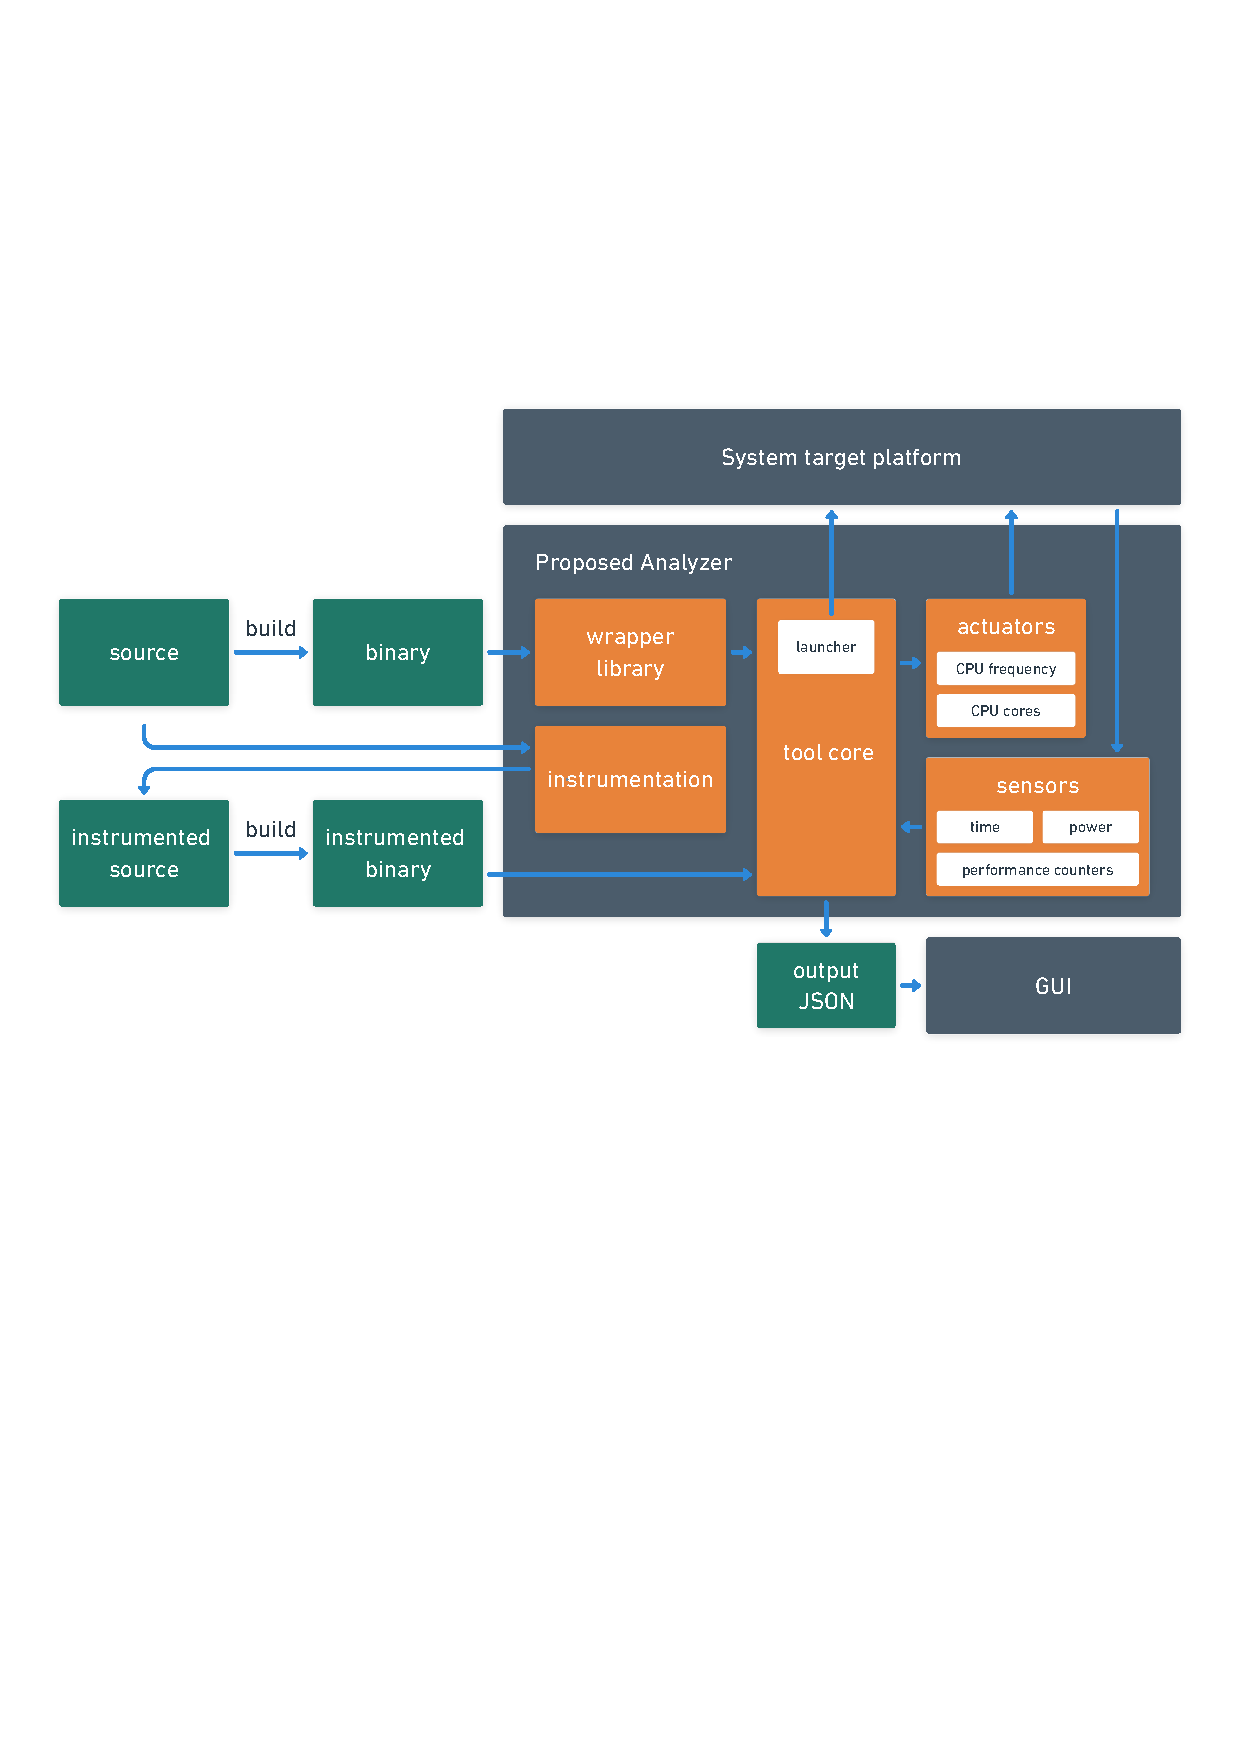
\includegraphics[scale=0.7]{pascalanalyzer/figures/designfeatures/pascal_philosophy.pdf}
	\caption{Architecture showing the interconnections of the central parts of the tool. Either binary (using the wrapper library) or an instrumented source code, the target application can be launched on the target platform by the tool core following the configuration parameters chosen by the user while deploying actuators/sensors. The resulting data collection is stored in Json file format for post analysis and visualization (GUI). \label{fig:pascal_architecture}}
\end{figure} 

\section{Instrumentation and Intrusiveness} \label{sec:instrumentation_and_intrusiveness}

The instrumentation module is one of the most crucial. In addition to automating the instrumentation, it determines the overload and level of intrusiveness of the instrumentation process. This module is designed to execute the fewest instructions possible in the most optimized manner. Currently, there is instrumentation support for C/C++ languages through shared libraries that work with either automatic or manual instrumentation. Manual instrumentation is preferred when it is necessary to examine the application program in specific code sections, regardless of the type of content. 

The manual instrumentation mode is implemented in three routines: one for initialization, another to mark the beginning of the region of interest ({\tt analyzer\_start}), and finally, a routine to mark the end of that region ({\tt analyzer\_stop}). The initialization routine is called when loading the library to create the necessary data structures and set up the data exchange communication. The routines {\tt analyzer\_start} and {\tt analyzer\_stop} identify threads in a region and store timestamps. These routines are implemented in such a way that only one thread at a time writes in a designated position of a two-dimensional array, thus ensuring thread safety and eliminating the necessity of locks.

The automatic instrumentation includes a routine allowing us to intercept the creation of threads via the {\tt LD\_PRELOAD} environment variable. This routine overwrites parts of an existing native library. In this manner, the functions responsible for thread spawning, such as {\tt pthread\_create} in the pthread library, {\tt GOMP\_parallel} (GCC implementation), {\tt \_\_kmpc\_fork\_call} (Clang implementation) in the OpenMP framework, and similar functions for other compilers, are intercepted to identify the parallel regions automatically. This approach is less intrusive than other tools, such as using a debugger interface with breakpoints or performing binary code instrumentation.

A key point of performance analysis tools, particularly important when analyzing real-time program execution, is that instrumentation must have a negligible impact on program behavior and execution time. Indeed, as mentioned in Section \ref{sec:pascal_architecture}, we support three types of sensors, each of which has a different degree of intrusion.
There is hardly any sensors intrusion at the start and then at the end of the program execution since it is simply the invocation of both data collection routines.

With sampling sensors, the degree of intrusion depends on the sampling rate and the total execution time of the application under study. Therefore, the intrusion needs to be assessed on a case-by-case basis with this type of sensor.

%It is fixed concerning the number of instructions and diverges with the number of threads. For example, suppose the user intends to analyze a parallelized region that is executed by four processing units. In that case, the execution time overhead is approximately equal to $4 \times T_{measurement}$, where $T_{measurement}$ corresponds to the time taken to perform a measurement, comprising the identification of events within the limits of the region involved in the measurement.

%The overhead for this example is the same when measuring two parallel regions with two cores and one parallel region with four cores. The \cref{lst:overheadsample1} and~\ref{lst:overheadsample2} present code snippets that correspond to the two scenarios mentioned and which, when analyzed using the tool, are therefore impacted by the same overhead.


The instrumentation overhead does not depend on the number of instructions or the runtime required to process the set of instructions to be analyzed. However, it varies according to the number of processing units used and measurements taken. To estimate the order of magnitude of the overhead ($T_{measurement}$), %MDPI: Is the italics necessary? Please carefully check and confirm. % yes
we measured recurring calls to the proposed sampling functions delimiting the regions in a simple benchmark code. This experiment was carried out in the same target architecture described in the experimental results of Section \ref{sec:casestudyarchitecture}, and the code structure is presented on Listing~~\ref{lst:overheadcode}.

\lstset{style=ccodestyle, frame=tb}

\begin{lstlisting}[label={lst:overheadcode}, language=C, caption={Code used to measure the overhead of instrumentation functions ({\tt analyzer\_start} and {\tt analyzer\_stop}) defined as $T_{measurement}$.}]
int main(int argc, char** argv) {
	get_time(begin);
	#pragma omp parallel for
	for (c=0; c<n_iterations; c++) {
		analyzer_start(1);
		usleep(1e4); // to simulate a simple operation
		analyzer_stop(1);
	} 
	get_time(end);
	time = begin-end;
}
\end{lstlisting}



The time required to execute $N$ %MDPI: Is the italic necessary? Please carefully check and confirm % yes
calls to the {\tt analyzer\_start} and {\tt analyzer\_stop} functions was obtained by the routine {\tt gettimeofday}, from the {\tt sys/time.h} library. The algorithm ran with 1 %MDPI: We used the scientific notations, please confirm. % ok
$\times~10^{4}$, 2 $\times~10^{4}$, 3 $\times~10^{4}$, 4 $\times~10^{4}$, 5 $\times~10^{4}$, and 1 $\times~10^{5}$ calls to the pair of functions, each test repetited ten times, and the mean, median, and variance values computed. \cref{fig:overhead} shows these results.

\begin{figure}[H]
\centering
\captionsetup{justification=centering}
\begin{subfigure}[b]{0.45\textwidth}	
	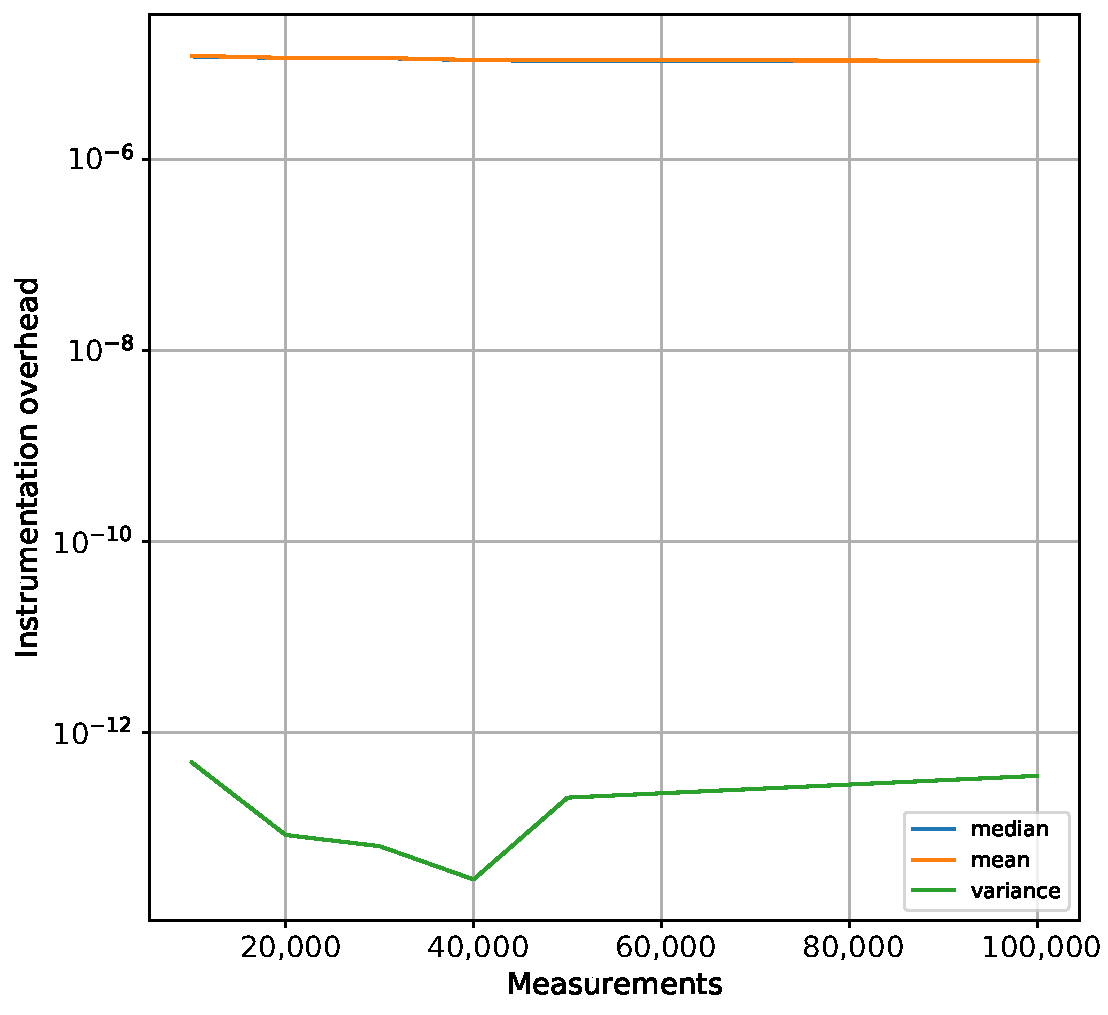
\includegraphics[width=\textwidth]{pascalanalyzer/figures/designfeatures/instrumentation_overhead_summary.pdf}
%	\caption{\centering}
	\label{fig:overhead_1}
\end{subfigure}
%
\begin{subfigure}[b]{0.46\textwidth}
	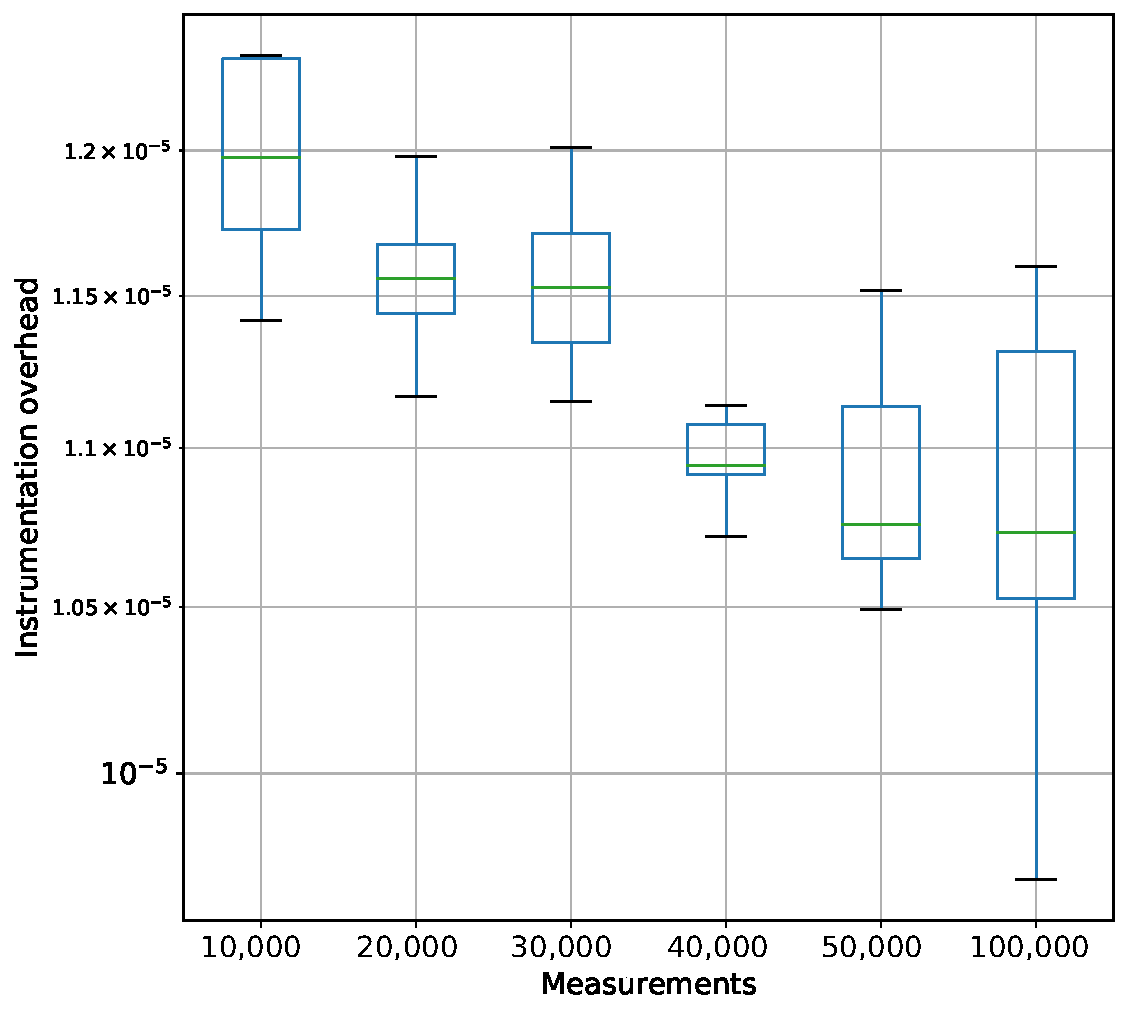
\includegraphics[width=\textwidth]{pascalanalyzer/figures/designfeatures/instrumentation_overhead_boxplot.pdf}
%	\caption{\centering}
	\label{fig:overhead_2}
\end{subfigure}
\caption{Measuring variance of the time to single instrumentation, 
	%MDPI: 1. For this figure, please use the scientific notations.
	%          2. Please add commas to numbers in the Ox axis of the figures, e.g.: 20,000 30,000 40,000 etc. - CHANGED
	i.e., a call to {\tt analyzer\_start} and {\tt analyzer\_stop} while varying the number of measurements. (\textbf{a}) Time consumed from sampling a region one time in seconds. %MDPI: We moved the explanations of subfigures here, please confirm.
	(\textbf{b}) Box plot showing the statistics of the sampling time of a single region.}
\label{fig:overhead}
\end{figure}

In Figure \ref{fig:overhead}a, we can see the mean, median, and variance of the time for a single call to our instrumentation function while varying the number of calls/measurements. The Figure \ref{fig:overhead}a complements these results showing the variance in each execution. %From these results, we can approximate the average value of $T_{measurement}$ to be $4e^{-6}$ seconds in this system. In other words, for each one million measurements, an overhead of approximately four seconds is added to the total program execution time.

\cref{tab:overhead} shows the results from the same experiment above comparing the time with and without the analyzer. We can observe that proportional impact (overhead) was constant while the number of interactions increased. \cref{tab:overhead} also presents the data referring to the simulation using the TAU profiling tool. For this simulation, we replaced the analyzer directives with the time measurement directives ({\tt TAU\_PROFILE\_START} and {\tt TAU\_PROFILE\_STOP}) of TAU, which allowed us to approximate the measurement and analysis conditions. 

\begin{table}[H]
\caption{Instrumentation overhead estimation varying the number of samples collected for TAU and~Analyzer.}
\label{tab:overhead}
%\centering
\newcolumntype{C}{>{\centering\arraybackslash}X}
\begin{tabularx}{\textwidth}{CCCCCC}\toprule
	\multirow{2}{*}{\vspace{-6pt}\textbf{Iterations}} & \multicolumn{3}{c}{\textbf{Time (s)}} & \multicolumn{2}{c}{\textbf{Overhead (\%)}} \\ \cmidrule{2-6}
	& \textbf{Real Time} & \textbf{TAU} & \textbf{Analyzer} & \textbf{TAU} & \textbf{Analyzer} \\ \midrule
	10,000	& 100.933	& 100.992	& 101.053	& 0.058	& 0.118 \\
	20,000	& 201.863	& 201.980	& 202.094	& 0.057	& 0.114 \\
	30,000	& 302.797	& 302.977	& 303.142	& 0.059	& 0.114 \\
	40,000	& 403.738	& 403.978	& 404.176	& 0.059	& 0.108 \\
	50,000	& 504.675	& 504.959	& 505.212	& 0.056	& 0.106 \\
	100,000	& 1009.359	& 1009.927	& 1010.432	& 0.056	& 0.106 \\ \midrule
\end{tabularx}
\end{table}

\textls[-20]{From the results, it is possible to see that the tool proposed in this work has a higher overhead than that presented by the TAU, but the analysis capabilities are distinct. TAU adds the individual runtime of each thread to define the execution time of a parallel region. This strategy does not consider the simultaneous action of threads in processing instructions and can count the same period of time more than once, damaging a precise measurement of the parallel region. The analyzer works around this problem because the intersection periods are counted just once. In this sense, although the TAU has lower overhead, a scalability analysis depends on a more accurate measurement like the one proposed in this work.}
\newpage
Varying the number of threads impacts the cost of instrumentation. As shown in \mbox{\cref{tab:overhead2}}, there is a trend for the percentage of overhead to increase concerning the application's runtime. However, it is also possible to see that this increase is negligible, considering the exponential increase in the number of threads. The increase in the processing load, on the other hand, has a beneficial impact on the relationship between execution time and the percentage of overhead. This behavior occurs because the runtime will increase with the greater need for processing, and the overhead will only change if the number of threads is also changed.

%The longer the execution time elapsed in each measurement, the smaller is the proportional impact of $T_{measurement}$ on the analysis as shown in Table .
%(9.181-9.142)/10000 = 0.0039s/Iteration
%(91.81-91.42)/100000 = 0.0000039s/Iteration
%100*(9.181-9.142)/9.181 = 0.4247 %over
%100*(91.81-91.42)/91.81 = 0.4247 %over
%The instrumentation overhead generated when measuring a region is located in the time of the outermost region. 
%This means that the execution time indicated by the tool for a region is only influenced by the instrumentation when there are more internal analysis regions. 
%In practice, the implementation strategy used in this tool offers the user the possibility of verifying more precisely the performance of certain parts of the code.


% Please add the following required packages to your document preamble:
% \usepackage{multirow}
%\begin{table*}
%\centering
%\caption{Overhead estimation varying the number of samples collected}
%\label{tab:overhead}
%\begin{tabular}{rrrrrrr}
%\midrule
%\multirow{2}{*}{Iterations} & \multicolumn{2}{c}{Time (s)} & \multicolumn{3}{c}{Time %estimation of single instrumentation (s)} & \multirow{2}{*}{Overhead (\%)} \\ %\cmidrule{2-6}
% & without analyzer & with analyzer & median %& average & variance & \\ \midrule
%10000 & 9.14 & 9.18 & 4.05e-06 & %4.03e-06 & 2.40e-14 & 0.44 \\
%20000 & 18.28 & 18.36 & 4.03e-06 & %4.04e-06 & 1.24e-14 & 0.44 \\
%30000 & 27.43 & 27.54 & 3.88e-06 %& 3.88e-06 & 1.35e-14 & 0.42 \\
%40000 & 36.57 & 36.72 & 3.89e-06 %& 3.90e-06 & 2.22e-14 & 0.43 \\
%50000 & 45.71 & 45.91 & 3.94e-06 %& 3.93e-06 & 2.52e-14 & 0.43 \\
%100000 & 91.42 & 91.81 & 3.93e-06 %& 3.90e-06 & 2.10e-14 & 0.43 \\ \midrule
%\end{tabular}
%\end{table*}

\begin{table}[H]
\caption{Instrumentation overhead while varying the number of threads with the number of samples fixed to one million.}
\label{tab:overhead2}
%\centering
\newcolumntype{C}{>{\centering\arraybackslash}X}
\begin{tabularx}{\textwidth}{CCCC}\toprule
	\multirow{2}{*}{\vspace{-6pt}\textbf{Threads}} & \multicolumn{2}{c}{\textbf{Time (s)}} & \multirow{2}{*}{\vspace{-6pt}\textbf{Overhead (\%)}} \\ \cmidrule{2-3}
	& \textbf{Direct} & \textbf{with Analyzer} \\ \midrule
	1 & 1009.360 & 1010.430 & 0.107 \\
	2	& 504.733	 & 505.374	 & 0.127 \\
	4	& 252.399	 & 252.742	 & 0.135 \\
	8	& 126.215	 & 126.390	 & 0.138 \\
	16	& 63.109	 & 63.199 & 0.143 \\ \bottomrule
\end{tabularx}
\end{table}

For pluggable sensors, overhead is generally not a concern as they run on a separate thread and have very low CPU usage, which presents only a few scenarios where they can cause interference.

\textls[-30]{One of these scenarios is where the application needs all the machine's resources at the same time that we have sensors that can respond faster than the processing speed at a given sample rate. In this case, the overhead would be directly associated with the sample rate and how the system handles concurrency. In general, this is rarer to happen in HPC (High-performance computing) since it would require an application with a perfect linear scaling.}

Another possible scenario is I/O overhead, where some network, disk, or memory resource becomes unavailable due to high sensor usage. However, this scenario is even rarer as sensors seldom produce data that quickly and, in all the performed tests, this was not close to being an issue.
	
\section{Features and Usage} \label{sec:features_and_usage}

The analyzer is a simple and easy-to-use tool that allows the user to understand the general behavior of a program before investing in efforts that require in-depth and sometimes longer-term analysis. However, to meet the objectives that best match the needs and resources of the user, the tool provides functionalities to parameterize the measurement process. Among the main ones are:
\begin{enumerate}
	\item Automated execution and deployment of parameterized code, actuators, and sensors
	%Automated code execution with different actuators and sensors saving time of a manual process.
	\item Automated low-overhead binary code instrumentation.
	\item No need of the source code or to recompile, unless the user desires it. 
	%Automated instrumentation in the binary with low overhead eliminating the need to access source code or recompile.
	\item Flexible user-defined observation regions: analysis of contexts within and beyond parallel regions.
	%The flexibility to identify specific observation regions: which allows the analysis of contexts beyond the blocks of instructions defined as parallel.
	\item Automatic instrumentation of parallel and remaining intermediate serial regions.
	%The ability to compute intermediate regions and automatically derive sensor values in certain parts of the program between user-defined regions. In scalability analysis, this becomes very useful since parallel regions can be instrumented automatically and the remaining regions can already be classified as serial, allowing the identification of all parts of the program.
	\item Aggregation, by region, of the collected metrics, which significantly reduces the amount of data stored on disk and RAM usage; useful in cases where it would be impossible to store information about all sensor events, such as the instrumentation of a for loop with billions of iterations. In this case it is possible to choose how to group the data either by mean, median, minimum or maximum values.
	\item Hierarchical regions: The proposed analyzer also facilitates the identification of aligned regions, enabling the identification of the calling hierarchy of inner regions and block analysis.
\end{enumerate}
\newpage
The tool can be used in the command line or via its API. The API provides calls to integrate sensors and actuators as shown in the Listing \ref{lst:pascal_api}.
%MDPI: Please provide the explanation % added in abbreviations


\lstset{style=pythonStyle,frame=tb}
\begin{lstlisting}[label={lst:pascal_api}, language=python, caption={Python script showing some API features provided by the tool, on how a custom run can be configured.}, captionpos=b]
from analyzer.run import Run
from analyzer.actuators import CPUFrequencies
from analyzer.actuators import CPUCores
from analyzer.sensors import RAPL
from analyzer.sensors import fingerprint
from itertools import product

lsensors = [
RAPL(), 
fingerprint(counters=["INSTRUCTIONS"])
]
cores = [
CPUCores(c) for c in range(1,32)
]
freqs = [
CPUFrequencies(2800000), 
CPUFrequencies(2600000)
]

# all combinations
configs = list(product(cores,freqs))
app = Run(application="a.out",
repetitions=10, 
instr_auto=True, 
sensors=lsensors)
app.run(configs)
app.savedata("out.json")
\end{lstlisting}



\section{Exported Data Structure} \label{sec:exported_data_structure}

The data collected by the tool is exported to a .json file and stored on disk. The data structure is divided into two large groups. One group contains information about the configuration parameters driving deployment and execution. The other includes the performance measurements. The data is grouped in keys representing the processed input, the number of processing elements used in the execution, and the simulation ID. Since the tool can perform the same configuration many times, a simulation ID distinguishes runs that use the same input and number of processing elements.


\cref{lst:datafile} presents an example file exported by the analyzer. There we can see the main parts of the exported structure, with the header where essential information about the system is written followed by the description of the collected data, where the list of actuators is presented as well as the specific type of information that was collected from the sensors. Finally the samples are presented separated by actuator configurations, and sensor type.

The keys and values in the .json file do not represent information that is easy for the user to identify and understand. However, it can be easily interpreted by a script or visualization software such as the PaScal Viewer~\cite{Silva2018}. The proposed tool provides a visualization module, responsible for interpreting and presenting data in an organized and user-friendly manner.

\lstset{style=jsonstyle, frame=tb}
\begin{lstlisting}[label={lst:datafile}, language=json, caption={Sample of exported data file showing the internal structure and organization of the data.}]
{
	"config": {
		****************** Header ******************
		"pkg": "./application", 
		"execdate": "00-00-0000_00:00:00",
		"kernel": "Linux-4.4",
		"command": "analyzer ...",
		"hostname": "host",
		...
		******** Data collected description ********
		"data_descriptor": {
			******** Mandatory collected values ********
			"values": [ 
			"start_time", "stop_time", ... 
			],
			************** Actuators list **************
			"keys": [ "A1", "A2" ...],
			********* Sensor data description **********
			"extras": {
				"regions": { ... }
				"sensors": { ... }
			}
		},
		"arguments": ["input_1", ...]
	},
	************** Data collected **************
	"data": {
		***** Actuator values separated by ";" *****
		"X;Y;Z": {
			********* Data collected by sensor *********
			"regions": { ... },
			"sensors": { ... },
			"start_time": ti,
			"stop_time": tf
		}
	}
}
\end{lstlisting}